%%
%% This is file `elsarticle-template-harv.tex',
%% generated with the docstrip utility.
%%
%% The original source files were:
%%
%% elsarticle.dtx  (with options: `harvtemplate')
%%
%% Copyright 2007, 2008 Elsevier Ltd.
%%
%% This file is part of the 'Elsarticle Bundle'.
%% -------------------------------------------
%%
%% It may be distributed under the conditions of the LaTeX Project Public
%% License, either version 1.2 of this license or (at your option) any
%% later version.  The latest version of this license is in
%%    http://www.latex-project.org/lppl.txt
%% and version 1.2 or later is part of all distributions of LaTeX
%% version 1999/12/01 or later.
%%
%% The list of all files belonging to the 'Elsarticle Bundle' is
%% given in the file `manifest.txt'.
%%
%% Template article for Elsevier's document class `elsarticle'
%% with harvard style bibliographic references
%% SP 2008/03/01

%\documentclass[11pt]{elsart}
\documentclass[11pt,onecolumn]{elsart3p}
%\documentclass[final,1p,times,11pt]{elsarticle}

%% Use the option review to obtain double line spacing
%% \documentclass[authoryear,preprint,review,12pt]{elsarticle}

%% Use the options 1p,twocolumn; 3p; 3p,twocolumn; 5p; or 5p,twocolumn
%% for a journal layout:
%% \documentclass[final,1p,times]{elsarticle}
%% \documentclass[final,1p,times,twocolumn]{elsarticle}
%% \documentclass[final,3p,times]{elsarticle}
%% \documentclass[final,3p,times,twocolumn]{elsarticle}
%% \documentclass[final,5p,times]{elsarticle}
%% \documentclass[final,5p,times,twocolumn]{elsarticle}

%% if you use PostScript figures in your article
%% use the graphics package for simple commands
%% \usepackage{graphics}
%% or use the graphicx package for more complicated commands
\usepackage{epsf,graphicx}
%% or use the epsfig package if you prefer to use the old commands
%% \usepackage{epsfig}

%% The amssymb package provides various useful mathematical symbols
\usepackage{amssymb,amsmath}
%% The amsthm package provides extended theorem environments
%% \usepackage{amsthm}

%% The lineno packages adds line numbers. Start line numbering with
%% \begin{linenumbers}, end it with \end{linenumbers}. Or switch it on
%% for the whole article with \linenumbers.
%% \usepackage{lineno}

\usepackage{color}
\newcommand{\vermell}{\textcolor{red}}

\journal{}

\hyphenation{op-tical net-works semi-conduc-tor}

\newtheorem{theorem}{Theorem}
\newtheorem{lemma}{Lemma}
\newtheorem{observation}{Observation}

\newenvironment{proof}{\vspace{1ex}\noindent{\bf Proof}\hspace{0.5em}}
    {\hfill\qed\vspace{1ex}}




\newcommand{\NACHO}[1]{\textcolor{red}{NACHO: #1}}
\newcommand{\TONI}[1]{\textcolor{red}{TONI: #1}}
\newcommand{\MARTA}[1]{\textcolor{red}{MARTA: #1}}

\begin{document}

\begin{frontmatter}

%% Title, authors and addresses

%% use the tnoteref command within \title for footnotes;
%% use the tnotetext command for theassociated footnote;
%% use the fnref command within \author or \address for footnotes;
%% use the fntext command for theassociated footnote;
%% use the corref command within \author for corresponding author footnotes;
%% use the cortext command for theassociated footnote;
%% use the ead command for the email address,
%% and the form \ead[url] for the home page:
%% \title{Title\tnoteref{label1}}
%% \tnotetext[label1]{}
%% \author{Name\corref{cor1}\fnref{label2}}
%% \ead{email address}
%% \ead[url]{home page}
%% \fntext[label2]{}
%% \cortext[cor1]{}
%% \address{Address\fnref{label3}}
%% \fntext[label3]{}

\title{Nearest and farthest spatial skyline queries under \\ multiplicative weighted Euclidean distances}
%\title{Nearest and farthest spatial skylines queries: \\ Euclidean vs multiplicative weighted Euclidean distances}

%% use optional labels to link authors explicitly to addresses:
%% \author[label1,label2]{}
%% \address[label1]{}
%% \address[label2]{}

\author{Marta Fort,  J. Antoni Sellar\`es \and Nacho Valladares}

%\address{}

\begin{abstract}
Let $P$ be a set of data points and $Q$ a set of query points in the plane. A nearest/farthest spatial skyline query retrieves the points of $P$ such that no other point of $P$ is simultaneously closer/farther to/from all the points of $Q$. The goal is to retrieve data points that are nearer/farther to/from at least one query point than all the other data points.
%A farthest spatial skyline query retrieves the points of $P$ such that no other point of $P$ is simultaneously farther to all the points of $Q$.
In this paper we study nearest and farthest spatial skyline queries when multiplicative weighted Euclidean distances are considered. Nearest spatial skyline queries are helpful to select interesting hotels of a city or appropriate locations to open a shop, while farthest spatial skyline queries are helpful in identifying desirable locations far away of garbage dumps, chemical plants or business competitors. We present a sequential and a parallel algorithm, to be run on the CPU and on a Graphics Processing Unit, respectively, for solving nearest/farthest spatial skyline queries. We also present the time and space complexity analysis of both algorithms, together with their theoretical comparison. Finally, we provide and discuss experimental results obtained with the implementation of the proposed sequential and a parallel algorithm.
\end{abstract}
\vspace{-1.5em}
\end{frontmatter}

%% \linenumbers

%% main text

\section{Introduction}

Spatial skylines are skylines on spatial attributes that are derived from the spatial distances between
the set of the data objects and a predefined set of query objects ...


\subsection{Spatial Skylines}

Given a set $P$ of $n$ data points and a set $Q$ of $m$ query points in the plane, the {\it nearest spatial skyline query} $NSSQ(P,Q)$ retrieves the points of $P$ such that no other point of $P$ is closer to all of the query points of $Q$ simultaneously. Let us see an example. A visitor of a trade fair identifies a set of city locations, say for example the central train station $c$ and the exhibition center venue $v$, and wants to select interesting hotels in terms of Euclidean distance. Accordingly, $Q = \{c,v\}$ and $P$ contains the hotels, considering the scenery depicted in Figure \ref{fig:NSSQExample1}, $P = \{h_1, \ldots, h_6\}$. We want to select the hotels $h$ that are no father simultaneously from $c$ and $v$ than any other hotel. Thus, hotels $h_1$, $h_2$ and $h_4$ are the most interesting hotels for the visitor and are the spatial skyline hotels of $P$ with respect to the selected city locations $c$ and $v$ that define $Q$.
%In this case $Q$ has cardinality two and thus the spatial skyline problem can be transformed to a traditional skyline problem of dimension 2.


\begin{figure}[!htp]
\begin{center}
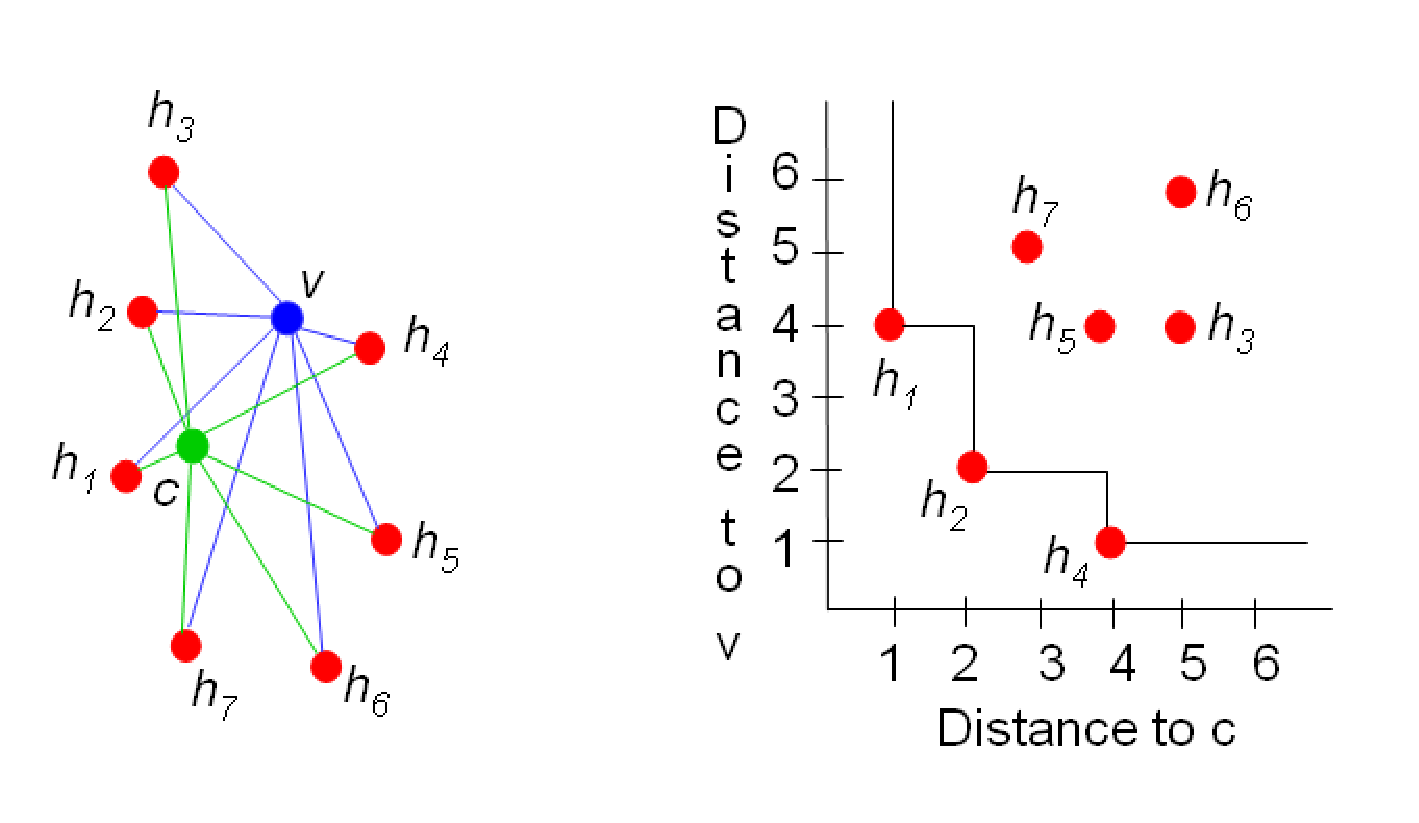
\includegraphics[width=9cm]{SSQExample1.eps}
\caption{Nearest spatial skyline hotels: $h_1$, $h_2$ and $h_4$. \TONI{Cal revisar Figura}}
\label{fig:NSSQExample1}
\end{center}
\end{figure}

There can be applications of this problem in other areas, such as: events organization, disaster management decisions or facility location, among others. For instance, suppose that the members of a multidisciplinary task team that work in different offices, need to meed together regularly. Let $Q$ be the set containing the locations of the offices where the members usually work and $P$ the set of potential locations for their weekly meetings. Among the locations contained in $P$ and according to $Q$, the best location for their weekly meeting is one of the skyline points of $P$. In disaster management, suppose that several residential buildings, defining the set $P$, must be evacuated because of several explosions or fires, defining $Q$. The first buildings to be evacuated according to their proximity to $Q$ are the spatial skyline buildings of $P$ with respect to the explosion or fire locations in $Q$. Finally, consider a business plan for opening a number of shops near a set of residential areas defining $Q$; the best locations for opening the new shops, among the potential locations defining the set $P$, are the spatial skyline locations of $P$ with respect to the residential areas in $Q$. Crisis management applications is another example: assume that a number of waterborne infectious disease cases were confirmed at different locations, people who live at spatial skyline places with respect to those locations should be alerted and examined first, because there might be higher possibility that these people may have been exposed to contagious water.

\vspace{1em}
Analogously, given a set $P$ of $n$ data points and a set $Q$ of $m$ query points in the plane, the {\it farthest spatial skyline query} $FSSQ(P,Q)$ retrieves the points of $P$ such that no other point of $P$ is farther from all of the query points of $Q$ simultaneously. Such queries are helpful in identifying spatial locations faraway from undesirable locations, e.g., unpleasant facilities (nuclear power plants, garbage dumps or chemical plants) or business competitors (hotels, restaurants). Figure \ref{fig:FSSQExample1} illustrates an example where among 10 potential locations for a new park, we aim at finding an optimal subset of locations, far from two query points in terms of Euclidean distance representing a chemical plant and a garbage dump. The most desirable locations for the park are the farthest spatial skyline locations $p_3$, $p_6$ and $p_7$.

\begin{figure}[!htp]
\begin{center}
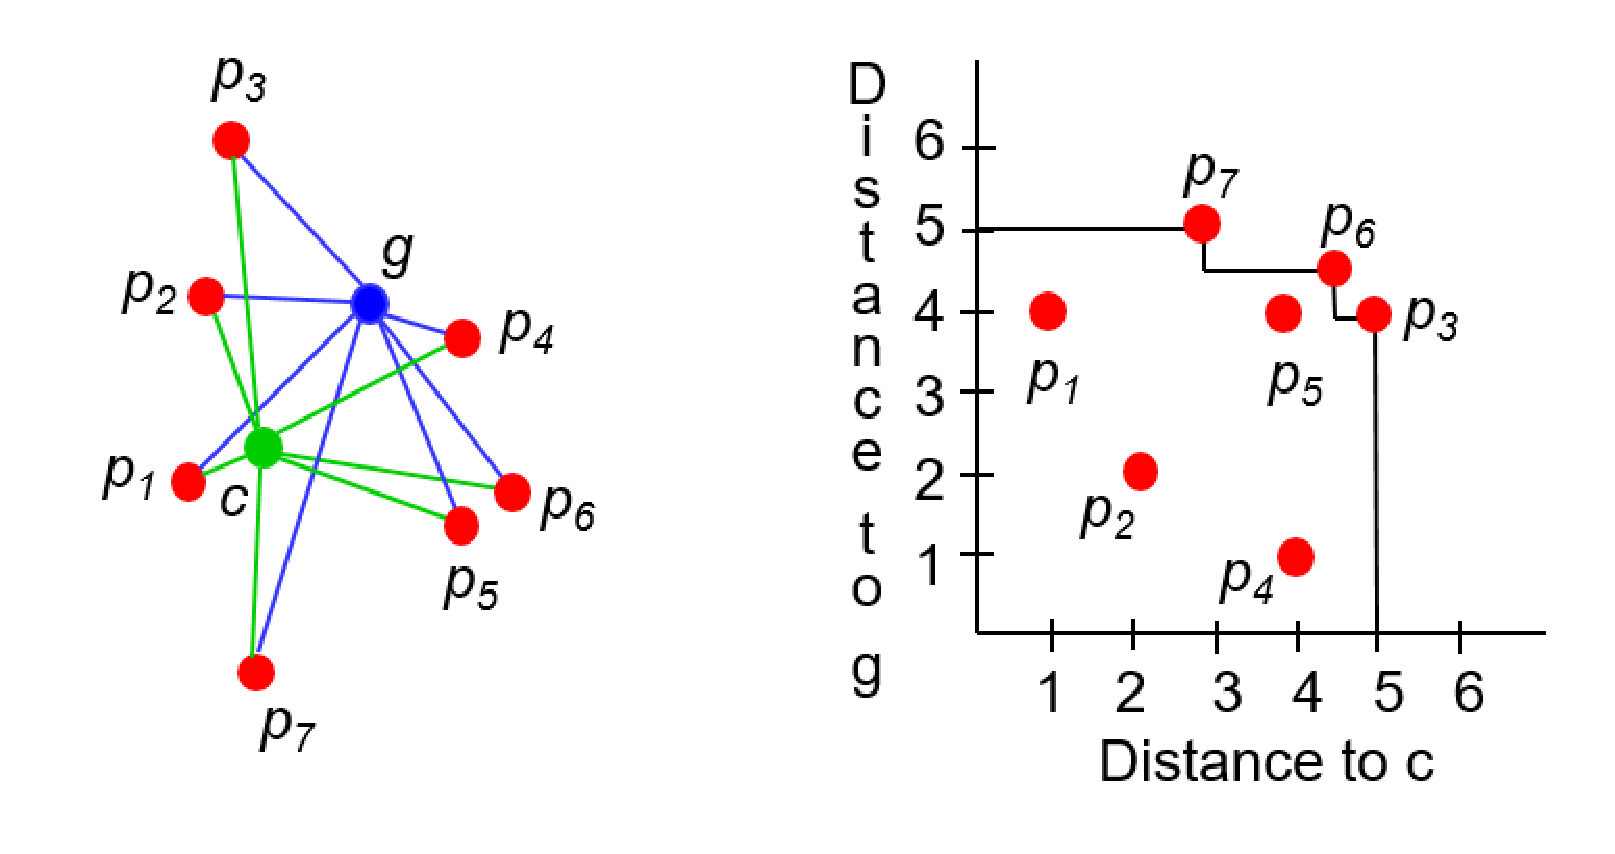
\includegraphics[width=9cm]{FarthestSkylineExample.eps}
\caption{Farthest spatial skyline parks: $p_3$, $p_6$ and $p_7$. \TONI{Cal revisar Figura}}
\label{fig:FSSQExample1}
\end{center}
\end{figure}

\vspace{1em}
 The skyline of the point set $P$ with respect to the query set $Q$ can be seen as the most �relevant� subset of $P$ with respect to $Q$. The query set $Q$ behaves as a set of constraints which each skyline point must satisfy.

\vspace{1em}
To the best of our knowledge, spatial skyline queries have been studied considering Euclidean and Manhattan distances, but ignoring the importance of data points of $P$ (e.g., hotels, shops, garbage dumps, business competitors). However, in practice the different importance of data points, either attractiveness or repulsiveness, must be taken into account. To this purpose, a weight is assigned to each point of $P$ to represent its importance. Experts take available information about different factors related to the data point, for instance the price and services of a hotel, and then aggregate these factors in a unique weight \cite{Dre94,DD02}.
To reflect that skyline points are determined depending on distance and importance, according to the model presented in \cite{BS97}, we associate to each data point of $P$ a weighted distance that is the product of the Euclidean distance and the inverse of the data point weight.

\subsection{Related work}

\subsection{Our contributions}

In this paper, we study, for the first time, nearest and farthest spatial skyline queries considering multiplicative weighted Euclidean distances. Since many of the geometric properties that are used by the approaches that solve spatial skyline queries under the Euclidean distance are not valid when considering  multiplicative weighted Euclidean distances, in working towards practical solutions, we exactly solve these queries with a GPU-parallel algorithm, under CUDA architecture, which is the main contribution of this paper for its efficiency, robustness and fast running times.

\subsection{Organization of the paper}

\section{Background}
\subsection{Multiplicative weighted Euclidean distances}

Let $P$ be a set of points in the plane.
Assume that each $p \in P$ is associated with a positive real weight $w_p > 0$. The {\it multiplicative weighted (Euclidean) distance} $d_p(q)$ from the location $p \in P$ to an arbitrary point $q$ is defined as $d_p(q)=(1/w_p)~d(p,q)$, where $d(p,q)$ denotes the {\it Euclidean distance} between points $p$ and $q$. Note that, the multiplicative weighted distances is non-metric, it is not symmetric and the triangle inequality does not hold because the weights change for each point.

\vspace{1em}
As an example, in Figure~\ref{fig:k-dissimilarity} we have a set $S$ of seven points and the squared query point $q$. In Figure~\ref{fig:k-dissimilarity}~a), where the Euclidean distance is considered, $S$ has one point at distance $u$ from $q$, two points at distance $2u$, three points at distance $3u$ and one point at distance $4u$. In Figure~\ref{fig:k-dissimilarity}~b), where multiplicative weighted distances are considered, the weights of the points of $S$ are the ones represented in brackets. In this case, $S$ has two points at weighted distance $u$ from $q$, one point at weighted distance $2u$, two points at weighted distance $3u$ and two points at weighted distance $4u$. Note that, in Figure~\ref{fig:k-dissimilarity}~b) the point placed on the smallest semi-circumference has a weighted distance of $4u$ with respect to $q$, meanwhile the point placed on the greatest semi-circumference is only at weighted distance $2u$ from $q$.

\begin{figure}[!htp]
\begin{center}
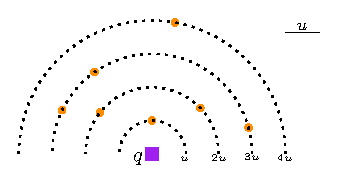
\includegraphics[width=0.4\linewidth]{knnExample.eps} \hspace{-0.5em} a) %k-dissimilarity.eps}
\qquad
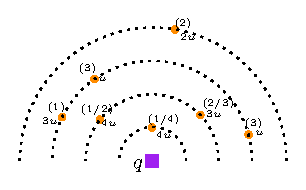
\includegraphics[width=0.4\linewidth]{knnExampleWeights.eps} \; b)
\caption{a) Euclidean distances; b) multiplicative weighted Euclidean distances.}
\label{fig:k-dissimilarity}
\end{center}
\end{figure}

\subsection{Bisectors and nearest regions}
%\vspace{1em}
For both, Euclidean and multiplicative weighted (Euclidean) distances, the bisector of points $p_i$ and $p_j$, denoted $b(p_i,p_j)$, is the locus of all points at identical distance to $p_i$ and $p_j$. It bisects the plane into two regions, $r(p_i,p_j)$ and $r(p_i,p_j)$. The region $r(p_i,p_j)$, the nearest region of the point $p_i$ with respect to the point $p_j$, consists of all points closer to $p_i$ than to $p_j$.

\vspace{1em}
{\bf Euclidean distance}. The bisector $b(p_i,p_j)$ is the straight line perpendicular to the line connecting $p_i$ and $p_j$ through their midpoint. The nearest region $r(p_i,p_j)$ is the open half-space $h(p_i,p_j)$ bounded by the bisector $b(p_i,p_j)$ that contains $p_i$.


\vspace{1em}
{\bf Multiplicative weighted distance}. The bisector of two points $p_i, p_j\in P$, the set of points $q$ such that $d_{p_i}(q)=d_{p_j}(q)$ or equivalently $d(p_i,q)/d(p_j,q)=w_{p_i}/w_{p_j}$, is a circle (Apollonius circle) if $w_{p_i} \ne w_{p_j}$ and a straight line otherwise.

\vspace{1em}
In the case where $w_{p_i} \ne w_{p_j}$, it is not difficult to prove that:

\vspace{1em}
a) The center of the bisector circle is the  point $c_{ij}=(w_{p_i}^2 p_j - w_{p_j}^2 p_i)/(w_{p_i}^2 - w_{p_j}^2)$;

\vspace{1em}
b) The points $p_i$,  $p_j$ and $c_{ij}$ are collinear, with $p_i$ and  $p_j$ on the same side of $c_{ij}$;

\vspace{1em}
c) The radius of the bisector circle is $r_{ij}=w_{p_i}w_{p_j} d(p_i,p_j)/|w_{p_i}^2 - w_{p_j}^2|$.

\iffalse
\vspace{1em}
Denote $b_{ij_1}$ and $b_{ij_2}$ the two intersection points between the bisector of $p_i$ and $p_j$ and the line through $p_i$ and $p_j$. Thus, it is $d(p_i,b_{ij_k})/d(p_j,b_{ij_k})=w_{p_i}/w_{p_j}$, $k=1,2$.
\vspace{1em}
d) We have $b_{ij_1}=(w_{p_i} p_j + w_{p_j} p_i)/(w_{p_i} + w_{p_j})$ and $b_{ij_2}=(w_{p_i} p_j - w_{p_j} p_i)/(w_{p_i} - w_{p_j})$;
\fi

\vspace{2em}

Examples of bisector circles $b(i,j)$ for fixed points $p_i$ and $p_j$ corresponding to different values of  $k=w_{p_i}/w_{p_j}$, where $k \ge 1$ is assumed without loss of generality, are shown in Figure \ref{fig:BisectorCircles}. The circles always surround point $p_j$. As $k$ grows the radius of the circles decreases and the center becomes close to $p_j$. On the contrary, as  $k$ diminish the radius of the circles increases and the center of the circles goes away from $p_j$. In the special case $k = 1$ ($w_{p_i}=w_{p_j}$), the bisector becomes a straight line (circle of infinite radius).
The nearest regions $r(p_i,p_j)$ and $r(p_j,p_i)$ are the exterior and interior of the bisector circles $b(i,j)$.

\vspace{2em}
\begin{figure}[!htp]
\begin{center}
\includegraphics[width=0.55\linewidth]{BisectorCircles.eps}
\caption{Bisector circles for several ratios $k=w_{p_i}/w_{p_j}$.}
\label{fig:BisectorCircles}
\end{center}
\end{figure}

\newpage
\section{Nearest and farthest skyline queries under multiplicative weighted Euclidean distances}

Let $P$ be a set of $n$ data points and $Q$ be a set of $m$ query points in the plane. We denote $CH(Q)$ the
convex hull of $Q$, and $E(Q)$ the set of vertices, called extreme points, of $CH(Q)$.

\vspace{1em}
All definitions that follow are consistent with prior literature \cite{LSAH10,SHA14,SSK09,YLIH13}.

\vspace{1em}
Given points $p_i, p_j \in P$, we say that $p_i$
{\it spatially dominates from near} [{\it far}] $p_j$ with respect to $Q$ if and only if
$d_{p_i}(q_k) \le d_{p_j}(q_k)$ [$d_{p_i}(q_k) \ge d_{p_j}(q_k)$] for every $q_k \in Q$, and $d_{p_i}(q_l) < d_{p_j}(q_l)$ [$d_{p_i}(q_l) > d_{p_j}(q_l)$] for some $q_l \in Q$.


\vspace{1em}
If  $CH(Q) \subset r(p_i, p_j)$ then $p_i$ spatially dominates from near $p_j$ and $p_j$ spatially dominates from far $p_i$ (see Figure \ref{fig:DomNotDom}).

\vspace{1em}
{\it Transitivity}. If $p_i$ spatially dominates from near [far] $p_j$ and $p_j$ spatially dominates from near [far] $p_k$, then $p_i$ spatially dominates from near [far] $p_k$.

\vspace{1em}
Point $p_j$ is {\it not spatially dominated from near} [{\it far}] by $p_i$ if and only $d_{p_j}(q_k) < d_{p_i}(q_k)$ [$d_{p_j}(q_k) > d_{p_i}(q_k)$] for some $q_k  \in Q$, or $d_{p_i}(q_k) = d_{p_j}(q_k)$ for all $q_k \in Q$. We also say that $p_i$ {\it does not spatially dominate from near} [{\it far}] $p_j$.

\vspace{1em}
If at least a point $q_k \in Q$ lies in $r(p_j, p_i)$ then $p_j$ is not spatially dominated from near by $p_i$ and
$p_i$ is not spatially dominated from far by $p_j$.

\vspace{1em}
A point $p_j \in P$ is a {\it nearest [farthest] spatial skyline point} with respect to $Q$ if and only if $p_j$ is not spatially dominated from near [far] by any other point of $P$.

\vspace{1em}
If for all $i \ne j$ at least a point $q_k \in Q$ lies in $r(p_j, p_i)$ [$r(p_i, p_j)$ ] then $p_j$ is a nearest [farthest] skyline point.

\vspace{1em} The goal of an {\it nearest} [{\it farthest}] {\it spatial skyline query} is to
retrieve the set $NSSQ(P,Q)$ [$FSSQ(P,Q)$] of all the nearest [farthest] spatial skyline points of
the set $P$ with respect to $Q$.

\begin{figure}[!htp]
\begin{center}
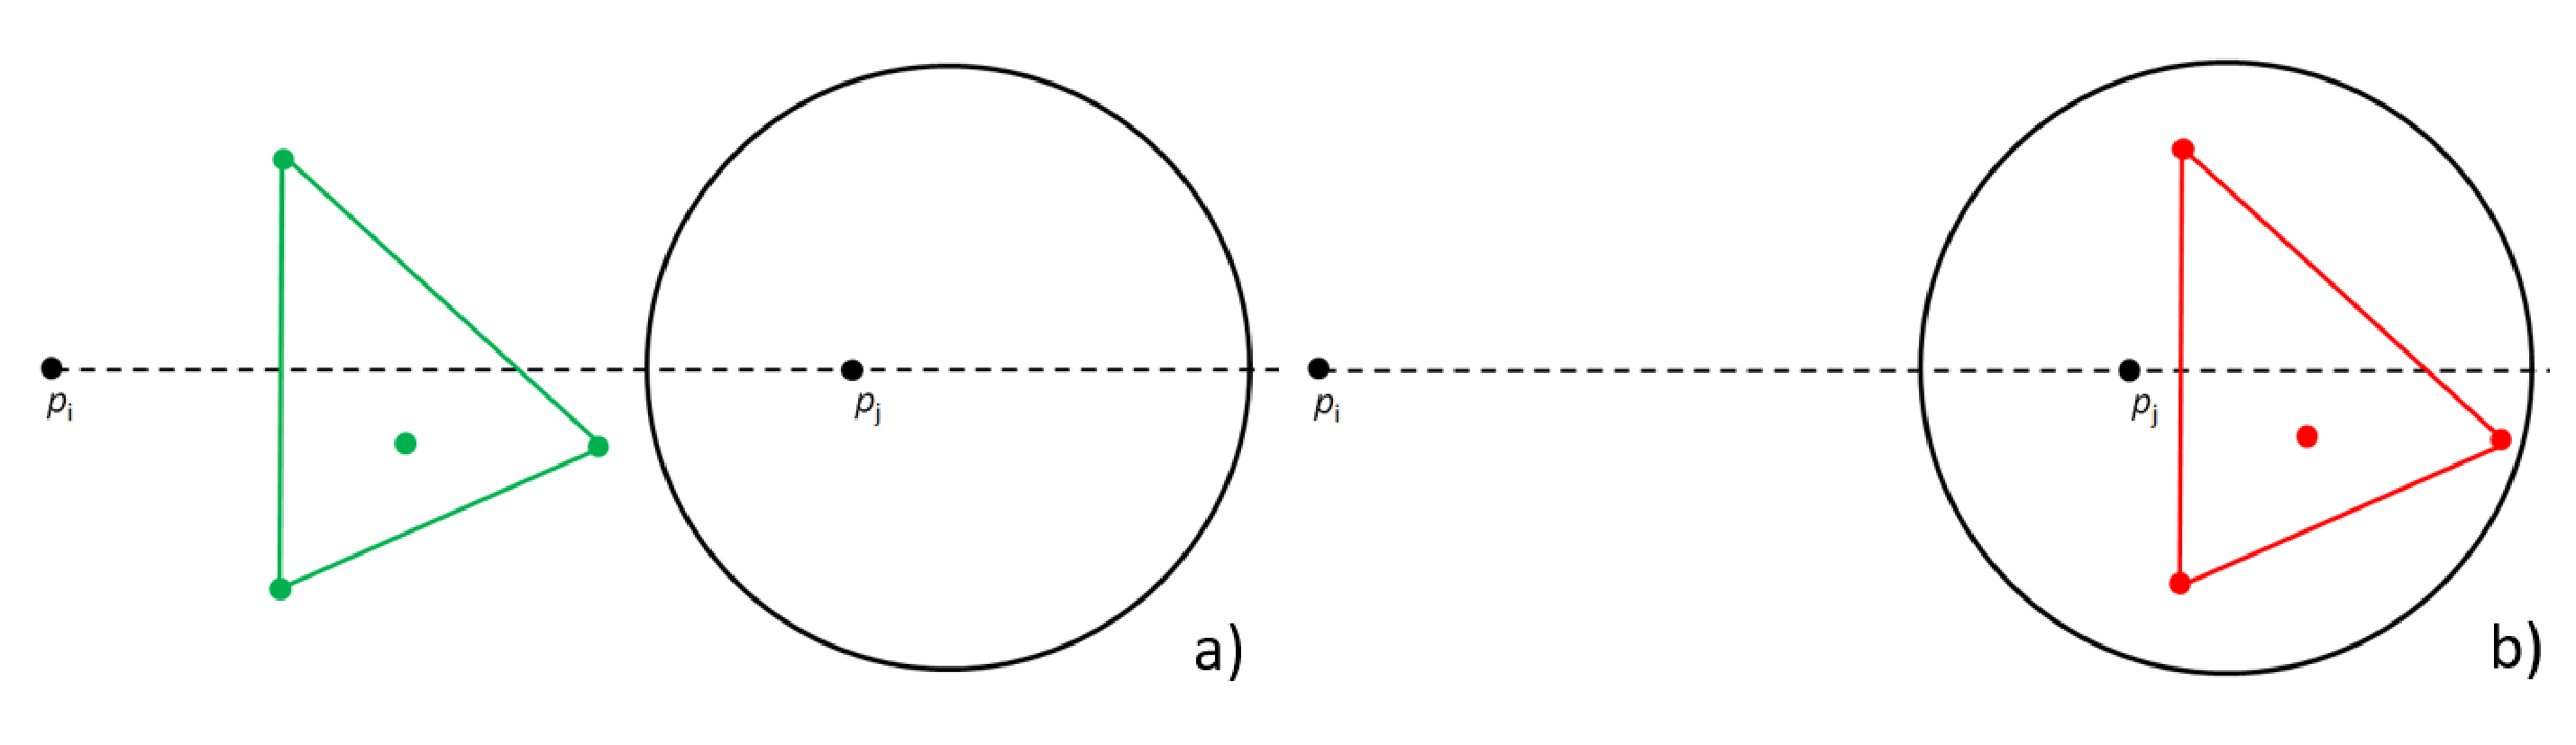
\includegraphics[width=0.8\linewidth]{DomNotDom.eps}
\caption{a) If $CH(Q) \subset r(p_i, p_j)$ then $p_i$ spatially dominates from near $p_j$ and $p_j$ spatially dominates from far $p_i$; b) If $CH(Q) \subset r(p_j, p_i)$ then $p_j$ spatially dominates from near $p_i$ and $p_i$ spatially dominates from far $p_j$.}
%\vspace{-0.5em}
\label{fig:DomNotDom}
\end{center}
\end{figure}


\newpage
\subsection{Nearest and farthest skylines properties: Euclidean vs multiplicative weighted Euclidean distances}

Many geometric properties observed for nearest and farthest skylines under the Euclidean distance no longer hold under
multiplicative weighted Euclidean distances.

\vspace{1em}
The following Lemmas 1-4 are valid for the Euclidean distance (see \cite{LSAH10,SSK09,YLIH13} for proofs):

\vspace{1em}
\begin{lemma} The set of nearest [farthest] skyline points of $P$ respect to $Q$ depends only on $E(Q)$. \label{lemma:NOnlyE}
\end{lemma}

\vspace{1em}
\begin{lemma} The bisector of two points in $P$ intersects $CH(Q)$ if and only if they do not spatially dominate from near [far] each other. \label{lemma:NIntBisectorCH}
\end{lemma}

\vspace{1.em}
\begin{lemma} If $E(Q) \subset r(p_i, p_j)$ then $p_i$ spatially dominates from near $p_j$ [$p_j$ spatially dominates from far $p_i$].
\label{lemma:NIntHalfSpaceCH}
\end{lemma}

\vspace{1em}
\begin{lemma} Any point $p \in P$ that is inside $CH(Q)$ is a nearest skyline point, but \vermell{may be or not} a farthest skyline point.
\label{lemma:NInsideCH}
\end{lemma}

\iffalse
\vspace{1em}
\begin{lemma} If the Voronoi region of a point of $P$ intersects with $CH(Q)$ then the point is a nearest skyline point. \TONI{Cal?}
\label{lemma:NVoronoi}
\end{lemma}
\fi

\iffalse
\vspace{1em}
\begin{lemma} The set of farthest skyline points of $P$ respect to $Q$
depends only on $E(Q)$. \label{lemma:FOnlyE}
\end{lemma}

\vspace{1em}
\begin{lemma} The bisector of two data points in $P$ intersects $CH(Q)$ if and only if they do not spatially dominate
from far each other. \label{lemma:FIntBisectorCH}
\end{lemma}

\vspace{1em}
\begin{lemma} If $E(Q) \subset r(p_i, p_j)$ then $p_j$ spatially dominates from far $p_i$.
\label{lemma:FIntHalfSpaceCH}
\end{lemma}

\vspace{1em}
\begin{lemma} A point of $P$ inside $CH(Q)$ \vermell{may not be} a farthest skyline point.
\label{lemma:FInsideCH}
\end{lemma}

\vspace{1em}
\begin{lemma} If the Voronoi region of a point of P intersects with $CH(Q)$ then the point does not
dominate from far any other point of $P$. \TONI{Cal?}
\label{lemma:FVoronoi}
\end{lemma}
\fi

\vspace{1em}
However, previous Lemmas 1-4 do not hold for Multiplicative weighted Euclidean distances, as follows from Observations 1-4:

\vspace{1em}
\begin{observation} The set of nearest [farthest] skyline points of $P$ respect to $Q$
\vermell{does not depend} only on $E(Q)$ (see Figure \ref{fig:NFOnlyE} a)). \label{obs:NFOnlyE}
\end{observation}

\vspace{1em}
\begin{observation} The bisector of two points in $P$ may intersect $CH(Q)$ while one of the points spatially dominates from near [far] the other (see Figure \ref{fig:NFIntBisectorCH} a) [Figure \ref{fig:FFIntBisectorCH} a)]). \label{observation:FIntBisectorCH}
\end{observation}

\vspace{1em}
\begin{observation} It may be that $E(Q) \subset r(p_i, p_j)$ while $p_i$ does not spatially dominates from near $p_j$ (see Figure \ref{fig:NFOnlyE} b)). It may be that $E(Q) \subset r(p_i, p_j)$ while $p_j$ does not spatially dominates from far $p_i$ (see Figure \ref{fig:NFOnlyE} d)).
\label{observation:NMayE}
\end{observation}

\vspace{1em}
\begin{observation} A point of $P$ inside $CH(Q)$ \vermell{may not be} a nearest [farthest] skyline point (see Figure \ref{fig:NFIntBisectorCH} b) [Figure \ref{fig:FFIntBisectorCH}  b)]).
\label{observation:FInsideCH}
\end{observation}

\iffalse
\vspace{1em}
\begin{observation}If the Voronoi region of a point of $P$ intersects with $CH(Q)$ then the point \vermell{may not be} a nearest skyline point (see Figure \ref{fig:NFIntBisectorCH} c)). \TONI{Cal?}
\label{observation::MNVoronoi}
\vspace{1em}
\end{observation}
\fi

\iffalse
\vspace{1em}
\begin{observation} The set of farthest skyline points of $P$ respect to $Q$
\vermell{does not depend} only on $E(Q)$ (see Figure \ref{fig:NFOnlyE} c)). \label{obs:FFOnlyE}
\end{observation}

\vspace{1em}
\begin{observation} The bisector of two points in $P$ may intersect $CH(Q)$ while one of the points spatially dominates from far the other (see Figure \ref{fig:FFIntBisectorCH} a)). \label{observation:FIntBisectorCH}
\end{observation}

\vspace{1em}
\begin{observation} It may be that $E(Q) \subset r(p_i, p_j)$ while $p_j$ does not spatially dominates from far $p_i$ (see Figure \ref{fig:NFOnlyE} d)).
\label{observation:FIntHalfSpaceCH}
\end{observation}

\vspace{1em}
\begin{observation} A point of $P$ inside $CH(Q)$ \vermell{may not be} a farthest skyline point (see Figure (see Figure \ref{fig:FFIntBisectorCH}  b)).
\label{observation:FInsideCH}
\end{observation}

\vspace{1em}
\begin{observation} If the Voronoi region of a point of $P$ intersects with $CH(Q)$ then the point may dominate from far an other point of $P$. (see Figure \ref{fig:FFIntBisectorCH} c)). \TONI{Cal?}
\label{observation:MNVoronoi}
\vspace{1em}
\end{observation}
\fi

\begin{figure}[!htp]
\begin{center}
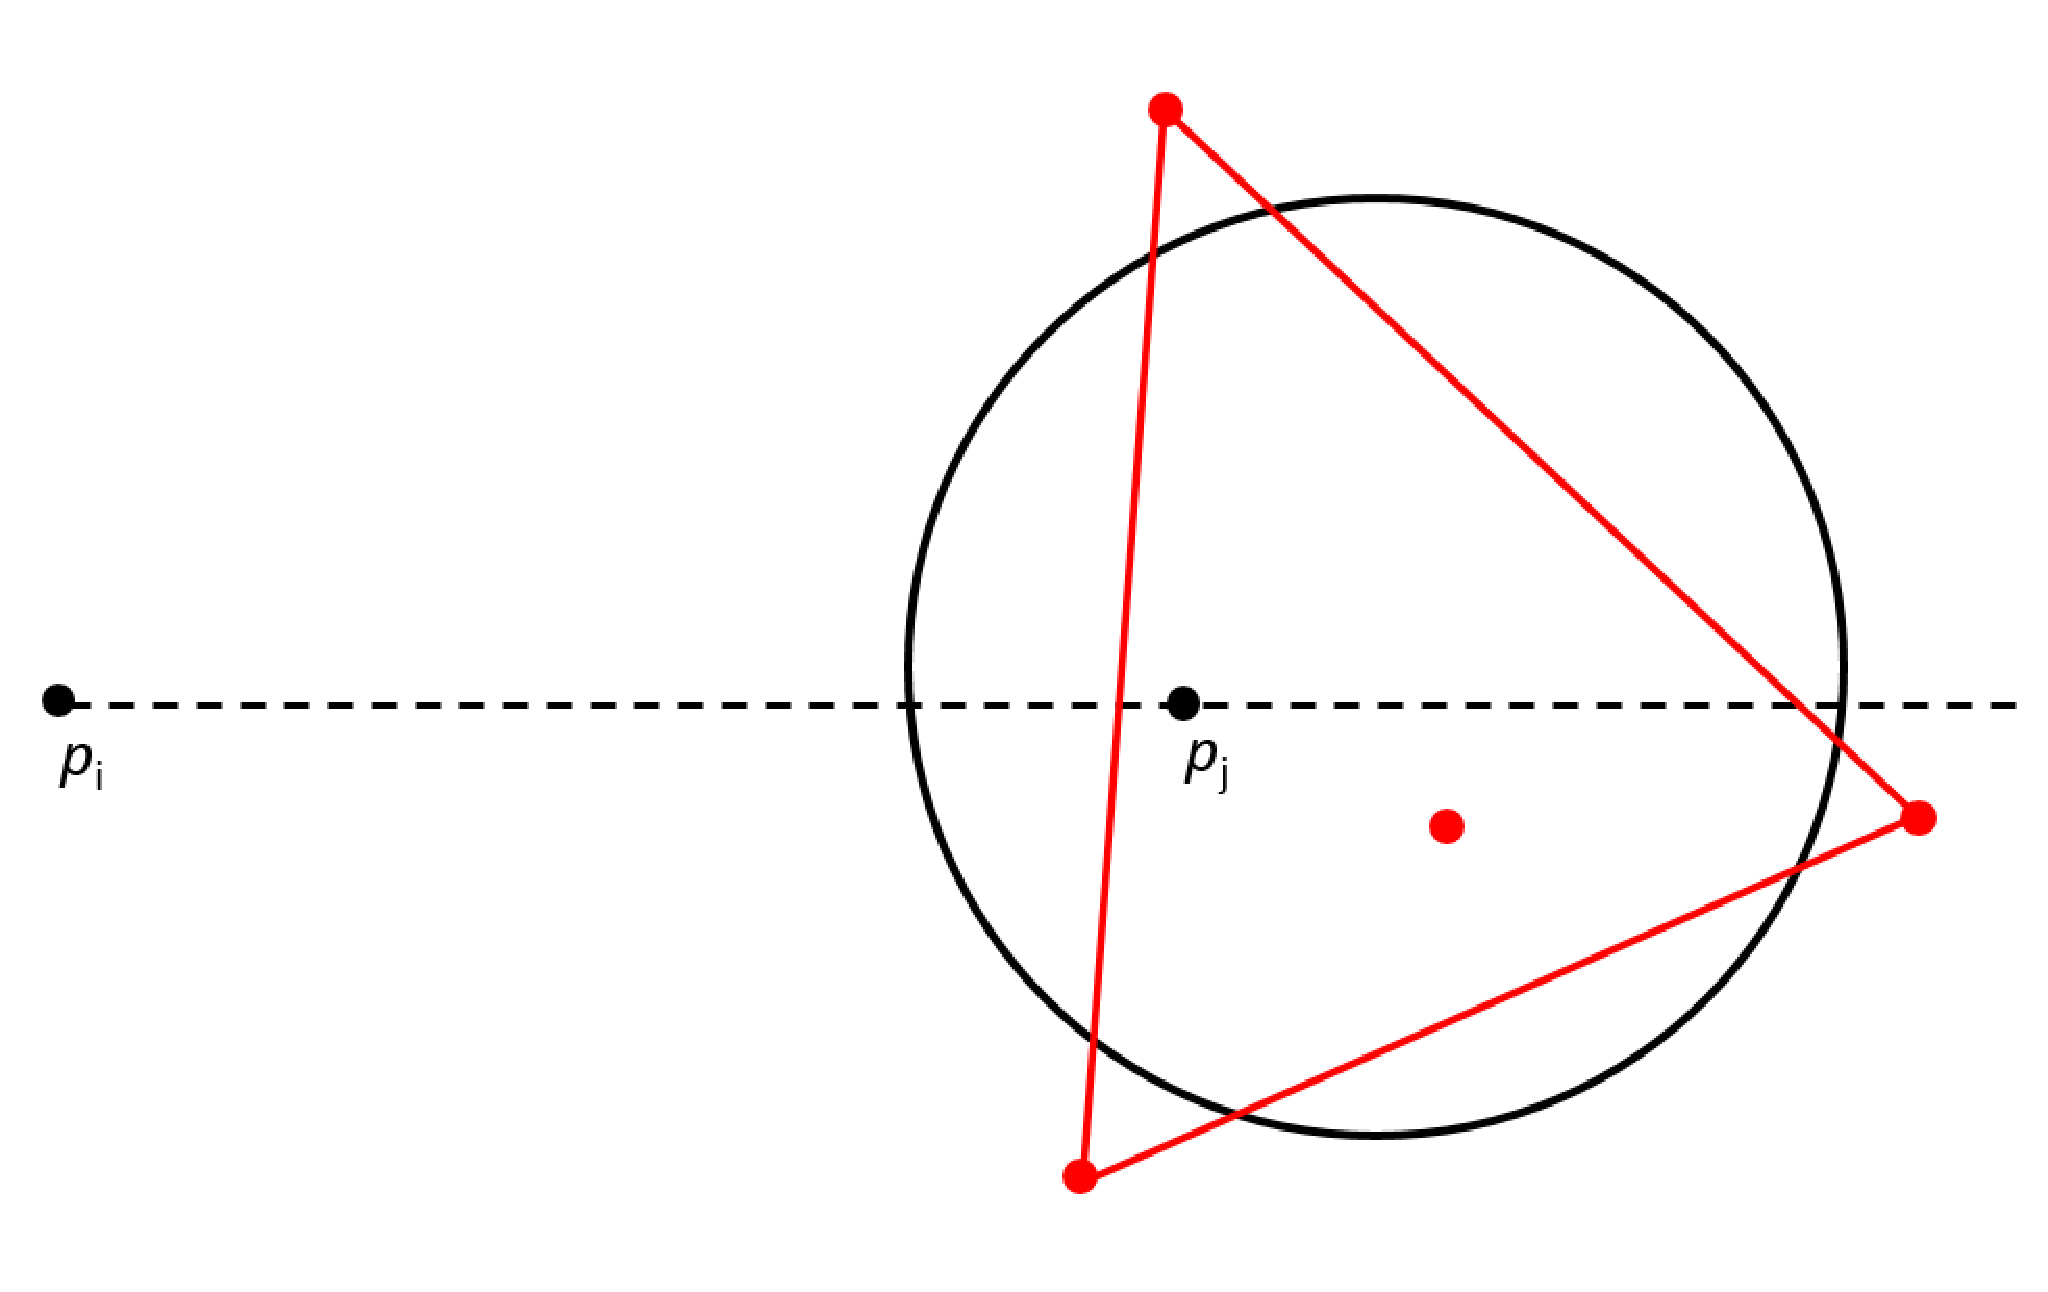
\includegraphics[width=0.4\linewidth]{NFOnlyE.eps}
\caption{a) Point $p_i$ dominates from near $p_j$ with respect to $E(Q)$, but $p_j$ is not dominated from near by $p_i$ with respect to $Q$. Point $p_j$ dominates from far $p_i$ with respect to $E(Q)$, but $p_i$ is not dominated from far by $p_j$ with respect to $Q$. b) We have $E(Q) \subset r(p_i, p_j)$, but $p_i$ does not spatially dominates from near $p_j$. We have $E(Q) \subset r(p_i, p_j)$, but $p_j$ does not spatially dominates from far $p_i$.}
\label{fig:NFOnlyE}
\end{center}
\end{figure}

\begin{figure}[!htp]
\begin{center}
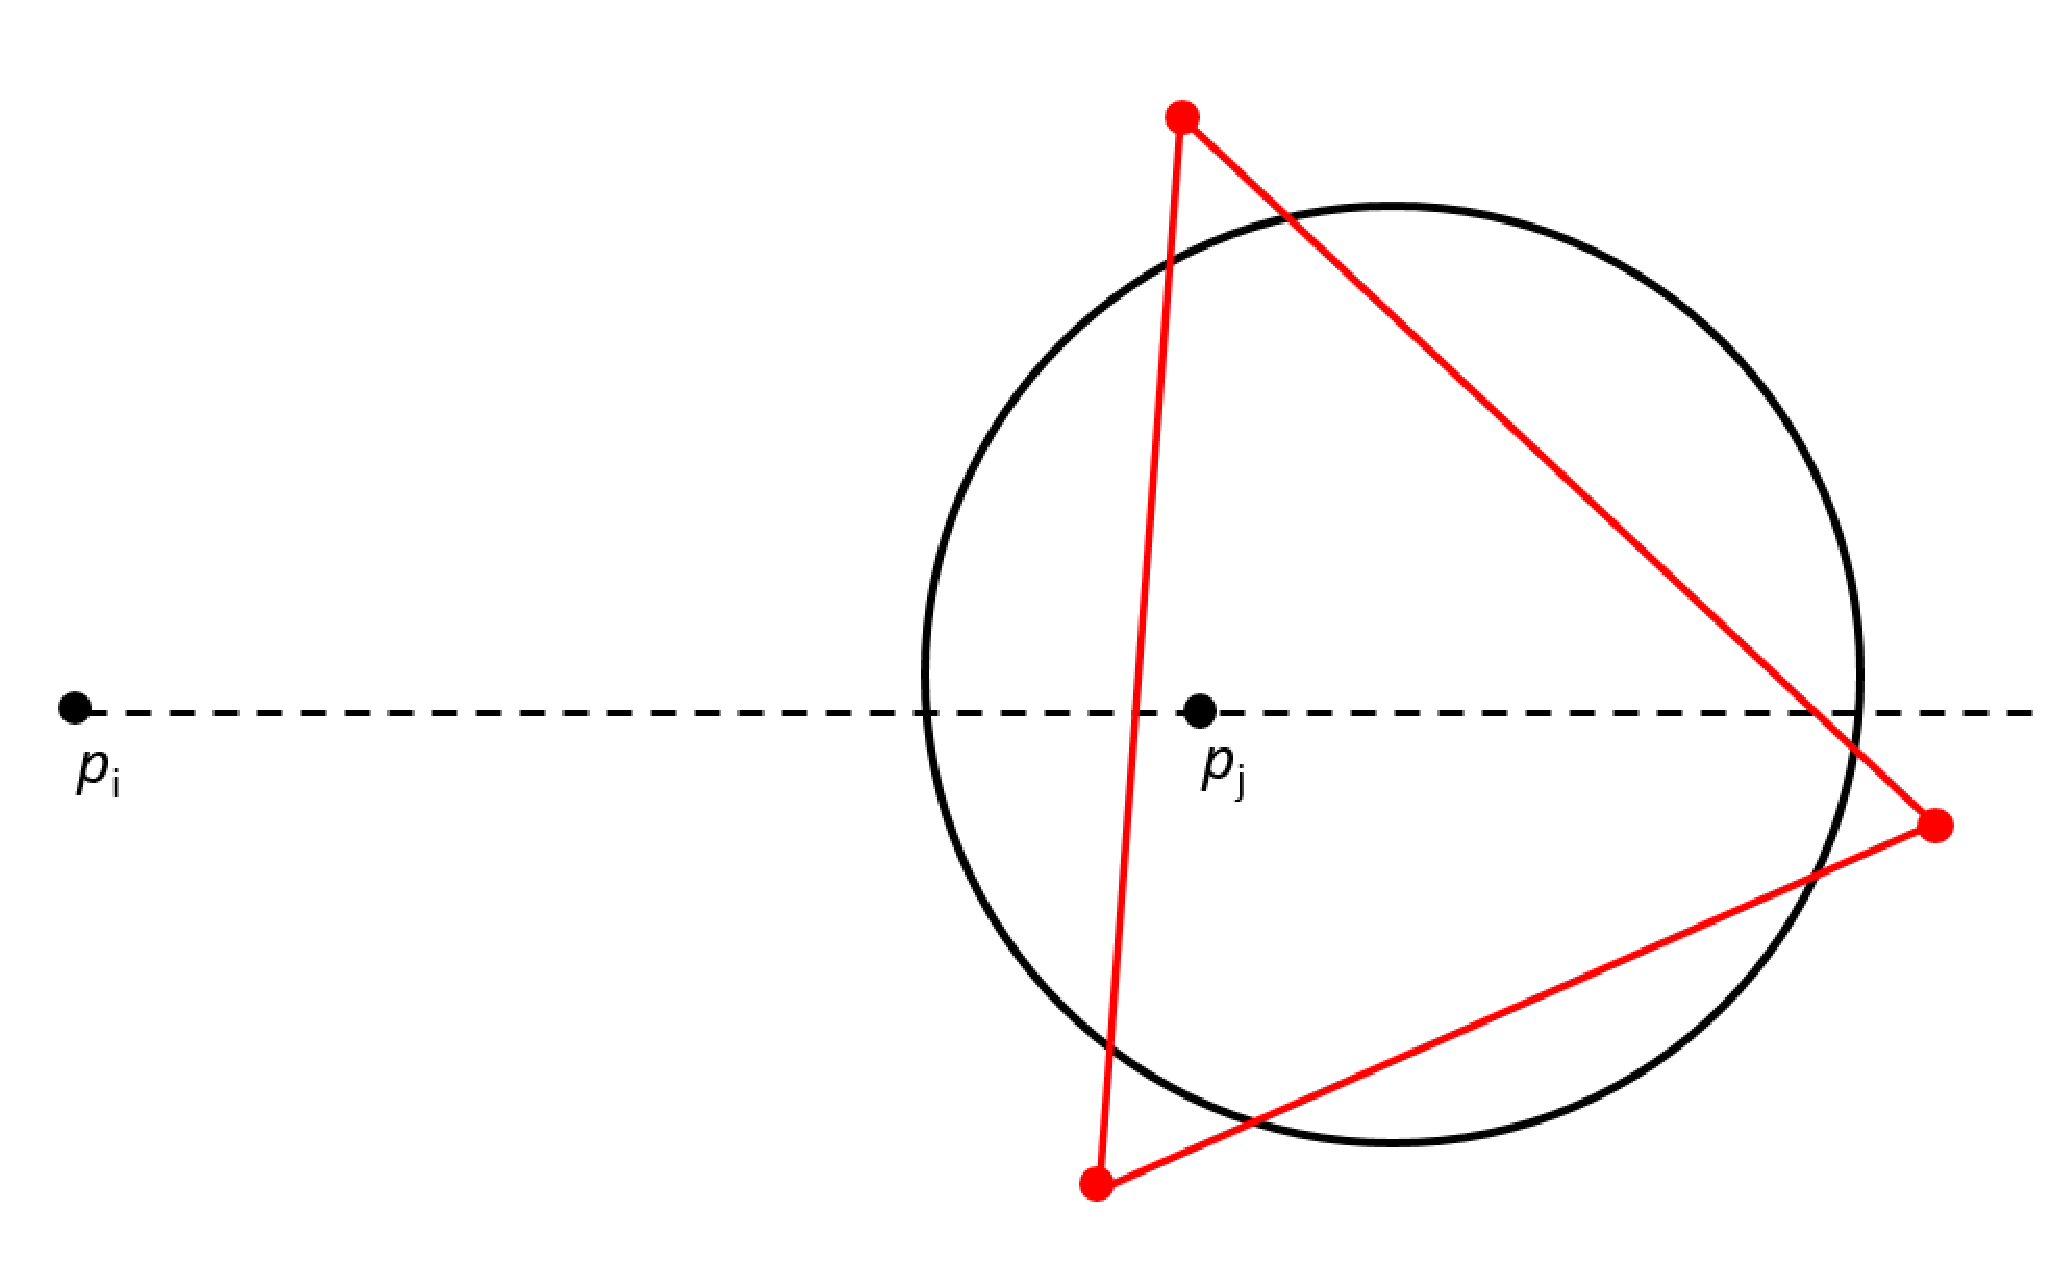
\includegraphics[width=0.4\linewidth]{NFIntBisectorCH.eps}
\caption{a) The bisector of $p_i$ and $p_j$ intersects $CH(Q)$, but $p_i$ dominates from near $p_j$. b) Point $p_j$  is inside $CH(Q)$ but it is not a nearest skyline point because $p_i$ dominates it from near.
%c) The Voronoi region of $p_j$ intersects with $CH(Q)$ but $p_j$ is not a nearest skyline point because $p_i$ dominates it from ner.
}
\label{fig:NFIntBisectorCH}
\end{center}
\end{figure}

\begin{figure}[!htp]
\begin{center}
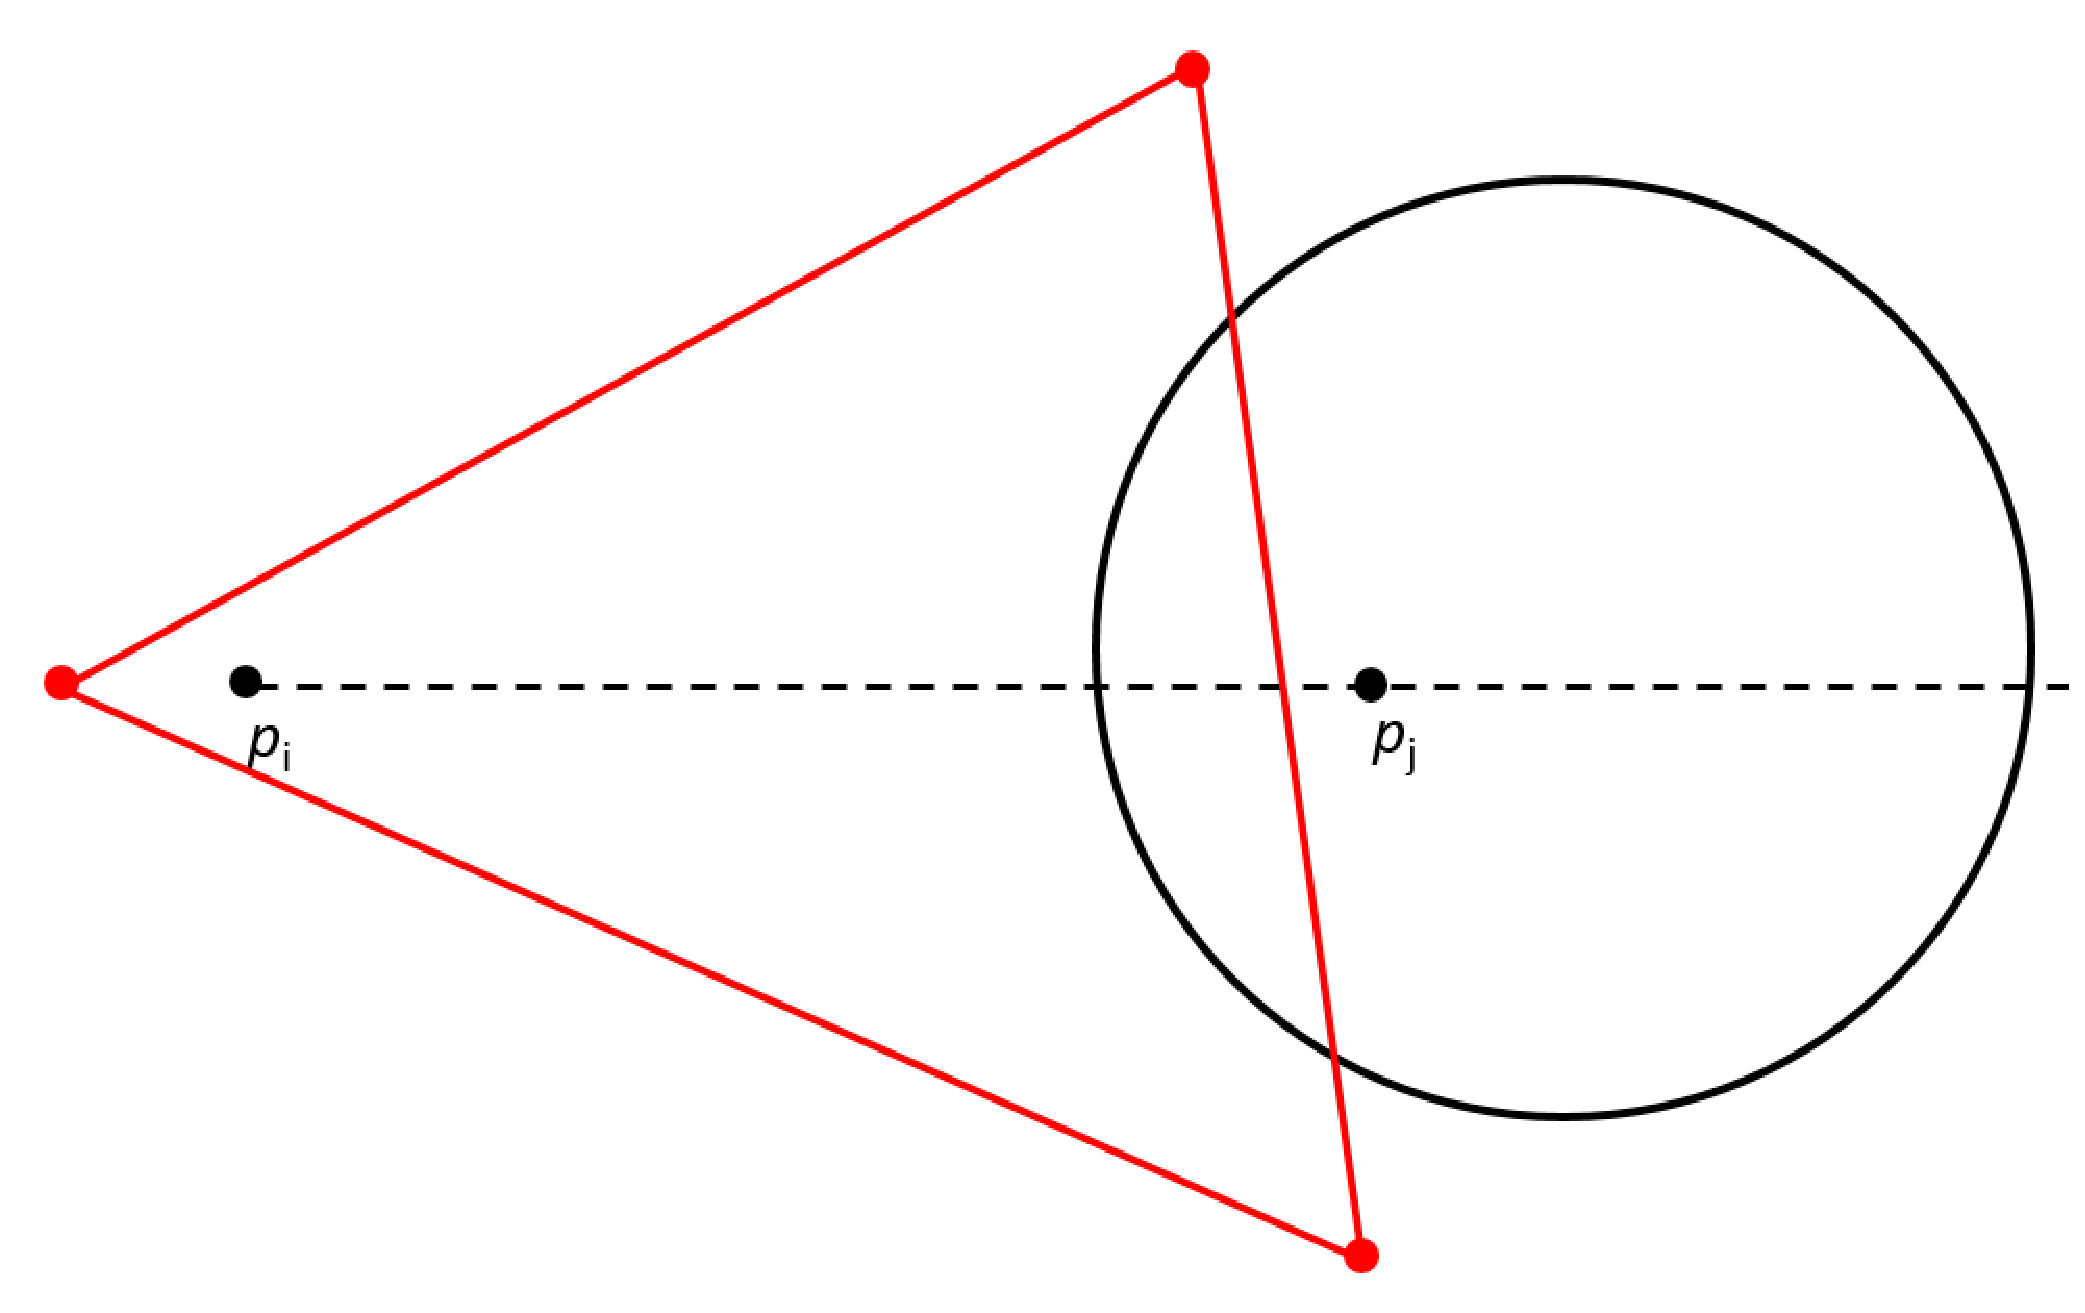
\includegraphics[width=0.4\linewidth]{FFIntBisectorCH.eps}
\caption{a) The bisector of $p_i$ and $p_j$ intersects $CH(Q)$, but $p_j$ dominates from far $p_i$. b) Point $p_i$  is inside $CH(Q)$ but it is not a farthest skyline point because $p_j$ dominates it.
%c) The Voronoi region of $p_j$ intersects with $CH(Q)$ and $p_j$ dominates from far $p_i$.
}
\label{fig:FFIntBisectorCH}
\end{center}
\end{figure}


\clearpage
\section{Retrieving nearest and farthest spatial skylines under the Euclidean distance}

{\it Ordenacio respecte un punt del convex hull}

\vspace{1em}
Spatial skyline query algorithms can be more efficient by pruning some $p_j$.

\vspace{1em}
Recordem, pels nearest, que:

- If  $CH(Q) \subset r(p_i, p_j)$ then $p_i$ spatially dominates from near $p_j$

- If at least a point $q_k \in Q$ lies in $r(p_i, p_j)$ then $p_i$ is not spatially dominated by $p_j$.

- A point $p_i \in P$ is a {\it nearest spatial skyline point} with respect to $Q$ if and only if $p_i$ is not spatially dominated by any other point of $P$.

- If for all $i \ne j$ at least a point $q_k \in Q$ lies in $r(p_j, p_i)$ then $p_j$ is a nearest skyline point.

o equivalentment:

- If there exist $i \ne j$  with $CH(Q) \subset  r(p_i, p_j)$ then $p_i$ spatially dominates from near $p_j$, thus $p_j$ is not a nearest skyline point.

\vspace{1em}
Idea: ordenem punts per distancia a un punt convex hull. Si $p_1$ abans $p_2$, llavors $p_2$ no domina $p_1$.


- Si $p_1$ i $p_2$ van abans que $p_3$ i $p_1$ domina $p_2$, llavors no necessitem comparar $p_3$ amb $p_2$. Hi ha dues possibilitats:

- $p_2$ domina $p_3$. LLavors per transitivat $p_1$ domina $p_3$, cosa que ja trobem al comparar $p_1$ i $p_3$, i $p_3$ s'elimina perque no pot ser skyline.

- $p_2$ no domina $p_3$. Pot passar que $p_1$ domini o NO a $p_3$. Si NO el domina llavors $p_3$ es skyline!

\vspace{1em}
Note that if a point is marked as a non-skyline point, it can be removed from the data for further computation.

\vspace{1em}
Pels farthest funciona pr�cticament igual!

If FOR ALL $i \ne j$ at least a point $q_k \in Q$ lies in $r(p_i, p_j)$  then $p_j$ IS A  farthest skyline point.

equival a

If THERE EXIST $i \ne j$  with $CH(Q) \subset  r(p_j, p_i)$ then $p_i$  spatially dominates from far $p_j$, thus $p_j$ IS NOT A  farthest skyline point.

\newpage
\section{Proposed algorithms for solving nearest and farthest spatial skyline queries under Multiplicative weighted Euclidean distances}

\begin{minipage}{0.47\textwidth}
\begin{tabular}{p{0.94\textwidth}}
{\bf Euclidean distance}

\vspace{1em}
1) Compute $E(Q)$ and replace $Q$ by $E(Q)$

\vspace{1em}
2) Obtain the set $P_i$ of points interiors to $CH(Q)$ and identify them as nearest skyline points

\vspace{1em}
3) Obtain the set $P_e$ of points exteriors to $CH(Q)$. Initially all points of $P_e$ are marked as nearest skyline points. Then, using the process described below, when we find that a point is dominated by another point it is marked as non nearest skyline point.

\vspace{1em}
4.1) analitzem totes les parelles fins a determinar que un no es skyline (\vermell{es pot fer servir el Lemma \ref{lemma:NVoronoi}?}). Les parelles han de ser de $P_e$ x $P_i$ i de $P_e$ x $P_i$. Farem primer $P_e$ x $P_e$ i despres $P_e$ x $P_i$. Quan agafem una parella (p,q) de $P_e$ x $P_e$ mirem si p domina a q i si q domina a p, pero quan agafem $P_e$ x $P_i$ nomes ho mirem si q domina a p ja que q ja sabem que es skyline i per tant p no el dominara.

\vspace{1em}
4.1.1) per testejar la parella (p,q) considerem la mediatriu de segment pq i anem testejant punts de E(Q) \vermell{(precisar)} fins a trobar-ne un que estigui a cada banda de la mediatriu o a determinar que tots estan al mateix costat. En aquest cas el que els te tots al seu costat domina a l'altre i per tant l'altre no sera skyline i es desmarca com a skyline potencial. Aquest ja no cal descartar-lo, nomes cal mirar si aquest en domina a un altre per descartar l'altre.

\end{tabular}
\end{minipage}
\begin{minipage}{0.47\textwidth}
\begin{tabular}{p{0.94\textwidth}}
{\bf Multiplicative weighted distance}

\vspace{8em}
3) Initially all points of $P$ are marked as nearest skyline points. Then, using the process described below, when we find that a point is dominated by another point it is marked as non nearest skyline point.

\vspace{2em}
4.1) analitzem totes les parelles fins a determinar que un no es skyline. Per a cada parella (p,q) de $P$ x $P$ mirem si p domina a q i si q domina a p.

\vspace{6em}
4.1.1) per testejar la parella (p,q) considerem el bisector del segment pq i anem testejant punts de Q fins a trobar-ne un que estigui a cada banda del bisector o a determinar que tots estan al mateix costat. En aquest cas el que els te tots al seu costat domina a l'altre i per tant l'altre no sera skyline i es desmarca com a skyline potencial. Aquest ja no cal descartar-lo, nom�s cal mirar si aquest en domina a un altre per descartar l'altre.
\end{tabular}
\end{minipage}




\newpage

\section{Algorithms farthest}

\begin{minipage}{0.47\textwidth}
\begin{tabular}{p{0.94\textwidth}}
{\bf Euclidean distance}

\vspace{1em}
1) Compute $E(Q)$ and replace $Q$ by $E(Q)$

\vspace{1em}
2) Obtain the set $P_i$ of points interiors to $CH(Q)$ and identify them as nearest skyline points

\vspace{1em}
3) Obtain the set $P_e$ of points exteriors to $CH(Q)$. Initially all points of $P_e$ are marked as farthest skyline points. Then, using the process described below, when we find that a point is dominated by another point it is marked as non farthest skyline point.

\vspace{1em}
4.1) analitzem totes les parelles fins a determinar que un no es skyline (\vermell{es pot fer servir el Lemma \ref{lemma:NVoronoi}?}). Les parelles han de ser de $P_e$ x $P_i$ i de $P_e$ x $P_i$. Farem primer $P_e$ x $P_e$ i despres $P_e$ x $P_i$. Quan agafem una parella (p,q) de $P_e$ x $P_e$ mirem si p domina a q i si q domina a p, pero quan agafem $P_e$ x $P_i$ nomes ho mirem si q domina a p ja que q ja sabem que es skyline i per tant p no el dominara.

\vspace{1em}
4.1.1) per testejar la parella (p,q) considerem la mediatriu de segment pq i anem testejant punts de E(Q) \vermell{(precisar)} fins a trobar-ne un que estigui a cada banda de la mediatriu o a determinar que tots estan al mateix costat. En aquest cas el que els te tots al seu costat domina a l'altre i per tant l'altre no sera skyline i es desmarca com a skyline potencial. Aquest ja no cal descartar-lo, nomes cal mirar si aquest en domina a un altre per descartar l'altre.

\end{tabular}
\end{minipage}
\begin{minipage}{0.47\textwidth}
\begin{tabular}{p{0.94\textwidth}}
{\bf Multiplicative weighted distance}

\vspace{8em}
3) Initially all points of $P$ are marked as farthest skyline points. Then, using the process described below, when we find that a point is dominated by another point it is marked as non farthest skyline point.

\vspace{2em}
4.1) analitzem totes les parelles fins a determinar que un no es skyline. Per a cada parella (p,q) de $P$ x $P$ mirem si p domina a q i si q domina a p.

\vspace{6em}
4.1.1) per testejar la parella (p,q) considerem el bisector del segment pq i anem testejant punts de Q fins a trobar-ne un que estigui a cada banda del bisector o a determinar que tots estan al mateix costat. En aquest cas el que els te tots al seu costat domina a l'altre i per tant l'altre no sera skyline i es desmarca com a skyline potencial. Aquest ja no cal descartar-lo, nom�s cal mirar si aquest en domina a un altre per descartar l'altre.
\end{tabular}
\end{minipage}

\section{Experimental results}\label{sec:ExpResults}

\section{Conclusions} \label{sec:Conclusions}

\section{Acknowledgments}
Work partially funded by the XXX project from MEC, Spain.
We also acknowledge NVIDIA Corporation for the donation of the Tesla K40 GPU.


\begin{thebibliography}{00}

\bibitem{BS97}
B.~Boots, R.~South, Modeling retail trade areas using
higher-order, multiplicatively weighted {V}oronoi diagrams,
Journal of Retailing 73(3) (1997) 519--536.

\bibitem{Dre94}
T.~Drezner, 1994. Optimal continuous location of a retail
facility, facility attractiveness, and market share: An
interactive model. Journal of Retailing. 70(1), 49--64.

\bibitem{DD02}
T.~Drezner, Z.~Drezner, 2002. Validating the Gravity-Based
Competitive Location Model Using Inferred Attractiveness. Annals
OR 111(1-4), 227--237.

\bibitem{LSAH10}
M.~Lee, W.~Son, H.~Ahn, and S.~Hwang, \emph{Spatial skyline queries: exact and
approximation algorithms}, GeoInformatica (2010).

\bibitem{SHA14}
W. Son, S.W. Hwang, H.K. Ahn, \emph{MSSQ: Manhattan Spatial Skyline Queries}, Inf. Syst. 40, 2014, pp.~67--83.

\bibitem{SSK09}
M.~Sharifzadeh, C.~Shahabi, and L.~Kazemi, \emph{Processing spatial skyline queries in both vector spaces and spatial network databases}, ACM Trans. Database Syst. \textbf{34} (2009), pp.~1--45.

\bibitem{YLIH13}
G-W. You, M-W. Lee, H. Im,S-W. Hwang, \emph{The Farthest Spatial Skyline Queries} Inf. Syst. 38, 2013, pp.~286--301.

\end{thebibliography}

\end{document}


\bibliographystyle{amsplain}

\begin{thebibliography}{00}

\bibitem{AKSU12} Afrati, F.N., Koutris, P., Suciu, D., Ullman, J.D,  \emph{Parallel
skyline queries}, Proc. ICDT, 2012, pp.~274�-284.

\bibitem{BAM13} Bogh, K.S., Assent, I., Magnani, M. Efficient, \emph{GPU-based skyline
computation}, Proc. DaMoN, 2013, pp.~X--Y.

\bibitem{BCP08}	I. Bartolini, P. Ciaccia, M. Patella, \emph{Efficient sort-based skyline evaluation},
ACM Trans. Database Syst.33(4), 2008, pp.~1--49.

\bibitem{BEKMRZZ13} T. Bernecker, T. Emrich, H.P. Kriegel, N. Mamoulis, M. Renz, S. Zhang, A. Z�fle, \emph{Spatial inverse query processing}, GeoInformatica 17(3), 2013, pp.~449--487.

\bibitem{BKS01} S.~B\"orzs\"onyi, D.~Kossmann, and K.~Stocker, \emph{The skyline operator},
Data Engineering, 2001. Proceedings. 17th International Conference on, 2001, pp.~421--430.

\bibitem{CCM13} J. Chomicki, P. Ciaccia, N. Meneghetti, \emph{Skyline queries, front and
back}, SIGMOD Record 42(3), 2013, pp.~6--18.

\bibitem{CJTTZ06} C.Y. Chan, H.V. Jagadish, K.L. Tan, A.K.H. Tung, Z.
Zhang,\emph{Finding k-dominant skylines in high dimensional
space}, SIGMOD Conference, 2006, pp.~503--514.

\bibitem{CL09} L. Chen and X. Lian. \emph{Efficient processing of metric skyline
queries}, IEEE Trans. on Knowl. and Data Eng., 21(3), 2009,
pp.~351�-365.

\bibitem{CLY12} W. Choi, L. Liu, and B. Yu, \emph{Multi-criteria decision making
with skyline computation}, IEEE Information Reuse and Integration,
2012, pp.~316--323.

\bibitem{CSL13} Y.C. Chung, I.F. Su, C. Lee, \emph{Efficient computation of
combinatorial skyline queries} Inf. Syst. 38(3), 2013,
pp.~369--387.

\bibitem{DS07} E. Dellis and B. Seeger, \emph{Efficient computation of reverse
skyline queries}, Proc. 33rd Inter. Conf. on Very Large Data
Bases, 2007, pp.~291--302.

\bibitem{FGJCML13} X. Feng, Y. Gao, T. Jiang, L. Chen, X. Miao and Q. Liu
\emph{Parallel k-Skyband Computation on Multicore Architecture},
APWeb 2013, LNCS vol. 7808, 2013, pp.~827--837.

\bibitem{FJZ09} D. Fuhry, R. Jin, D, Zhang, \emph{Efficient skyline computation in
metric space}, EDBT, 2009, pp.~1042--1051.

\bibitem{GSG07} P.~Godfrey, R.~Shipley, and J.~Gryz, \emph{Algorithms and analyses for
maximal vector computation}, The VLDB Journal \textbf{16} (2007), pp.~5--28.

\bibitem{GXI12} X. Guo, C. Xiao, Y. Ishikawa, \emph{Combination Skyline Queries}, LNCS
Vol. 7600, 2012, pp.~1--30.

\bibitem{HLKP10} A. Han, Z. Li, D. Kwon, and Y. Park, \emph{An Efficient Method for
Processing Reverse Skyline Queries over Arbitrary Spatial
Objects}, Proc. of Database Technology and Applications, 2010,
pp.~1--4.

\bibitem{HLKP14} A. Han, Z. Li, D. Kwon, and Y. Park, \emph{An Efficient Pruning
Method to Process Reverse Skyline Queries}, Journal of Information
Science and Engineering, Vol. 30 No. 2, 2014, pp.~XXX�-YYY.

\bibitem{HPP11} H. Im, J. Park, S. Park, \emph{Parallel skyline
computation on multicore architectures}, Inf. Syst. 36(4), 2011,
pp.~808--823.

\bibitem{HP12} H. Im, S. Park, \emph{Group skyline computation}, Inf. Sci.
Vol. 188, 2012, pp.~151--169.

\bibitem{JTEH07} W. Jin, A.K.H. Tung, M. Ester, J. Han, \emph{On Efficient
Processing of Subspace Skyline Queries on High Dimensional Data},
SSDBM, 2007, pp.~X--Y.

\bibitem{KLH09}  J. Kim, J. Lee, S.W. Hwang, \emph{Skyline View: Efficient Distributed Subspace Skyline Computation},
DaWaK'09, 2009, pp.~312--324.

\bibitem{KYZ11} K\"ohler, H., Yang, J., Zhou, X, \emph{Efficient parallel skyline
processing using hyperplane projections}, ISIGMOD Conference,
2011, pp.~85�-96.

\bibitem{LC08} X. Lian and L. Chen, \emph{Monochromatic and bichromatic reverse
skyline search over uncertain databases}, Proc. ACM SIGMOD Inter.
Conf. on Management of Data, 2008, pp.~213�-226.

\bibitem{LCH09} Z. Ling, L. Cuiping and C. Hong, \emph{Efficient computation of
reverse skyline on data stream}, Inter. Joint Conf. on
Computational Sciences and Optimization, 2009, pp.~735--739.

\bibitem{LGCLJ12} Liu, Q., Gao, Y., Chen, G., Li, Q., Jiang, T, \emph{On efficient
reverse k-skyband query processing}, DASFAA 2012, LNCS vol. 7238,
2012, pp.~544-�559.

\bibitem{LH14} J. Lee, S.W Hwang, \emph{Scalable skyline computation using a balanced pivot selection technique}, Inf. Syst. 39, 2014, pp.~1--21.

\bibitem{LLZLT10} K. C. K. Lee, W.C. Lee, B. Zheng, H. Li, Y. Tian, \emph{Z-SKY: an efficient skyline query processing framework based on Z-order}, VLDB J. 19(3), 2010, pp.~333--362.

\bibitem{LSAH10}
M.~Lee, W.~Son, H.~Ahn, and S.~Hwang, \emph{Spatial skyline queries: exact and
approximation algorithms}, GeoInformatica (2010).

\bibitem{LY09}
H. Lu, M-L. Yiu, \emph{Identifying the Most Endangered Objects from Spatial Datasets}, Proc. Scientific and Statistical Database Management SSDBM (2009) pp. 608--626

\bibitem{LY11} H. Lu, M.L. Yiu, \emph{On Computing Farthest Dominated Locations},
IEEE Transactions on Knowledge and Data Engineering, vol. 23, no. 6, 2011, pp.~928--941.

\bibitem{LPLSY10} J. Lim, Y. Park, J. Lee, D. Seo, and J. Yoo, \emph{An efficient
method for processing reverse skyline queries}, Proc. of Mobile
Congress, 2010, pp.~1--5.

\bibitem{LVDN14} S. Liknes, A. Vlachou, C. Doulkeridis and K. N�rvag,
\emph{APSkyline: Improved Skyline Computation for Multicore
Architectures}, DASFAA 2014, 2014, pp.~X--Y.

\bibitem{LZZL13} Q. Lin, Y. Zhang, W. Zhang and A. Li, \emph{Efficient general spatial
skyline operator}, World Wide Web 16(3), 2013, pp.~247--270.

\bibitem{MLW09} Man Leung Wong,
\emph{Parallel multi-objective evolutionary algorithms on graphics processing units}, GECCO'09, 2009, pp.~2515--2522.

\bibitem{PTFS05} Papadias, D., Tao, Y., Fu, G., Seeger, B,  \emph{Progressive skyline
computation in database systems.}, ACM Trans. Database Syst.
30(1), 2005, pp.~41�-82.

\bibitem{SCL10} I.F. Su, Y.C. Chung, C. Lee, \emph{Top-k Combinatorial Skyline
Queries} DASFAA, 2010, pp.~79--93.

\bibitem{SHA14} W. Son, S.W. Hwang, H.K. Ahn, \emph{MSSQ: Manhattan Spatial Skyline Queries}, Inf. Syst. 40, 2014, pp.~67--83.

\bibitem{SL10} T. Skopal and J. Lokoc, \emph{Answering Metric Skyline Queries by
PM-tree}, Proc. Dateso, 2010, pp.~22--37.

\bibitem{SM12} A. Siddique, Y. Morimoto, \emph{Efficient k-dominant Skyline
Computation for High Dimensional Space with Domination Power
Index}, Journal of Computers, Vol 7(3), 2012, 608-615,
pp.~608--615.

\bibitem{SSK09}
M.~Sharifzadeh, C.~Shahabi, and L.~Kazemi, \emph{Processing spatial skyline
  queries in both vector spaces and spatial network databases}, ACM Trans.
  Database Syst. \textbf{34} (2009), pp.~1--45.

\bibitem{VDK08} Vlachou, A., Doulkeridis, C., Kotidis, Y,  \emph{Angle-based space
partitioning for efficient parallel skyline computation},  Proc.
of SIGMOD, 2008, pp.~X--Y.

\bibitem{VN09} A. Vlachou, K. N�rv�g, \emph{Bandwidth-constrained distributed skyline computation}, MobiDE'09, 2009, pp.~17--24.

\bibitem{WAT13} Woods, L., Alonso, G., Teubner, J., \emph{Parallel computation of
skyline queries}, Proc. of FCCM, 2013, pp.~X--Y.

\bibitem{ZMC09} S. Zhang, N. Mamoulis, D.W. Cheung, \emph{Scalable skyline computation using object-based space partitioning} SIGMOD'09, 2009, pp.~483--494.

\bibitem{YLIH13} G-W. You, M-W. Lee, H. Im,S-W. Hwang, \emph{The Farthest Spatial Skyline Queries}
 Inf. Syst. 38, 2013, pp.~286--301.

\bibitem{YM09} M.L. Yiu, N. Mamoulis, \emph{Multi-dimensional top-k dominating queries}, VLDB J. 18(3), 2009, pp.~695--718.

\end{thebibliography} 